\documentclass[12pt]{article}
%Gummi|065|=)
\usepackage{amsmath, amsfonts, amssymb}
\usepackage[margin=0.5in]{geometry}
\usepackage{xcolor}
\usepackage{graphicx}

\newcommand{\off}[1]{}
\DeclareMathSizes{20}{30}{20}{18}

\newcommand{\two }{\sqrt[3]{2}}
\newcommand{\four}{\sqrt[3]{4}}
\newcommand{\red}{\begin{tikz}[scale=0.25]
\draw[fill=red, color=red] (0,0)--(1,0)--(1,1)--(0,1)--cycle;\end{tikz}}
\newcommand{\blue}{\begin{tikz}[scale=0.25]
\draw[fill=blue, color=blue] (0,0)--(1,0)--(1,1)--(0,1)--cycle;\end{tikz}}
\newcommand{\green}{\begin{tikz}[scale=0.25]
\draw[fill=green, color=green] (0,0)--(1,0)--(1,1)--(0,1)--cycle;\end{tikz}}

\usepackage{tikz}

\newcommand{\susy}{{\bf Q}}
\newcommand{\RV}{{\text{R}_\text{V}}}

\title{Worksheet: Lagrange Interpolation}
\author{John D Mangual}
\date{}
\begin{document}

\fontfamily{qag}\selectfont \fontsize{12.5}{15}\selectfont

\maketitle

\noindent There are functions which satisfy a bewildering number of constraints.  Or we might find in a paper, a the existence of a function - satisfying very reasonable constraints - which is nearly impossible to construct.  \\ \\
Let's try to find an $f(x)$ that passes through a few points.
\begin{itemize}
\item $f(0) = 1$
\item $f(1) = 2$
\item $f(2) = 2$
\item $f(3) = 3$
\item $f(4) = 0$
\end{itemize}
How will we find such a function?  Let's guess a structure for it:
$$ f(x) = a_0 + a_1 x + a_2 x^2 + a_3 x^3 + a_4 x^4 + a_5 x^5 $$
Next plug in the values $x = 0$, $x = 1$, etc to solve a system of simultaneous equations:
\begin{eqnarray*}
f(0) = 1 &=& a_0 + a_1 \times 0 + a_2 \times0^2 + a_3 \times0^3 + a_4\times 0^4 + a_5 \times0^5 \\
f(1) = 2 &=& a_0 + a_1 \times 1 + a_2 \times1^2 + a_3 \times1^3 + a_4\times 1^4 + a_5 \times1^5 \\
f(2) = 2 &=& a_0 + a_1 \times 2 + a_2 \times2^2 + a_3 \times2^3 + a_4\times 2^4 + a_5 \times2^5 \\
f(3) = 3 &=& a_0 + a_1 \times 3 + a_2 \times3^2 + a_3 \times3^3 + a_4\times 3^4 + a_5 \times3^5 \\
f(4) = 0 &=& a_0 + a_1 \times 4 + a_2 \times4^2 + a_3 \times4^3 + a_4\times 4^4 + a_5 \times4^5 
\end{eqnarray*}
The equation is solved in a standard way called \textbf{Lagrange Interpolation}
\begin{eqnarray*} f(x)
 &=& f(0)\; \frac{(x-1)(x-2)(x-3)(x-4)}{(0-1)(0-2)(0-3)(0-4)} \\
 &+& f(1)\; \frac{(x-0)(x-2)(x-3)(x-4)}{(1-0)(1-2)(1-3)(1-4)} \\
 &+& f(2)\; \frac{(x-1)(x-2)(x-3)(x-4)}{(2-0)(2-1)(2-3)(2-4)} \\
 &+& f(3)\; \frac{(x-1)(x-2)(x-3)(x-4)}{(3-0)(3-1)(3-2)(3-4)} \\
 &+& f(4)\; \frac{(x-1)(x-2)(x-3)(x-4)}{(4-0)(4-1)(4-2)(4-3)} 
\end{eqnarray*}
A little bit complicated to write down, we can set $x = 0, 1, 2, 3, 4$ and check it works.

\newpage

\noindent Not without artifacts\dots However, looks very good in some places!

\includegraphics{lagrange-01.png} \\ \\
We don't really know what is happending between the values of $x = 0$ and $x = 1$.  \\
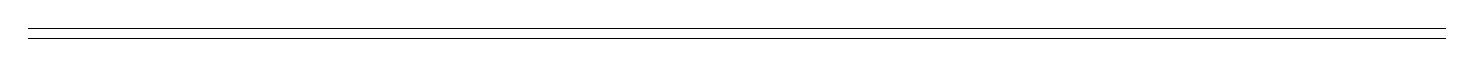
\begin{tikzpicture}
\draw (0,0)--(18,0);
\draw (0,-0.125)--(18,-0.125);
\end{tikzpicture} \\ \\
\textbf{NEXT} more constraint problems.  Maybe in two dimensions.

\newpage  

\begin{thebibliography}{}

\item \dots 

\end{thebibliography}

\end{document}